\documentclass{beamer}
\usetheme[block = fill, titleformat title = allcaps, titleformat subtitle  = smallcaps, background = light]{metropolis}           % Use metropolis theme
\usepackage{tikz-network}
\title{Municipal housing market structure as barrier to within-country migration}
\subtitle{A multilevel analysis for the Netherlands}
\date{\today}
\author{Thomas de Graaff}
\institute{Vrije Universiteit Amsterdam\\Department of Spatial Economics}
\begin{document}
\maketitle

\section{The problem}

  \begin{frame}{Contempory applied spatial economic research}
    	\begin{itemize}
    		\item 50--70\% of all research questions in spatial economics evolve around policy \alert{evaluation} or \alert{explaining} impact of \alert{isolated} variables 
    		\item Huge demand (firms \& government for research dealing with \alert{prediction} and \alert{assessing} total model performance
    		\item But, more than 90\% of all statistical analysie is done with basic applied econometrics using \alert{linear} models and \alert{fixed} effects
    	\end{itemize}
  \end{frame}

\begin{frame}{Prediction in gravity models}
	 \begin{figure}	

	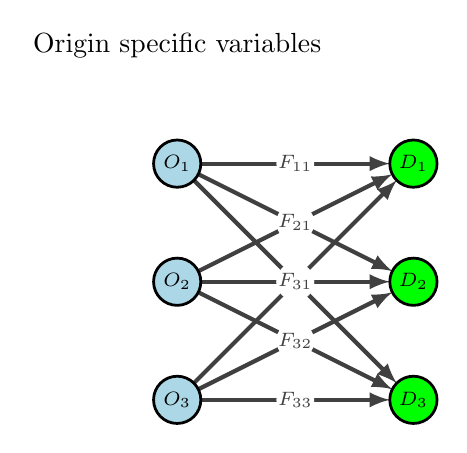
\begin{tikzpicture};
		
		\Text[y = 1.5]{Origin specific variables}
		
		\Vertex[label = $O_1$]{O1}
		\Vertex[label = $O_2$,y = -1.5]{O2}
		\Vertex[label = $O_3$, y = -3]{O3})
		
		\Vertex[label = $D_1$, x = 3, color = green]{D1}
		\Vertex[label = $D_2$, x = 3, y = -1.5, color = green]{D2}
		\Vertex[label = $D_3$, x = 3, y = -3, color = green]{D3})
		 
		\Edge[label=$F_{11}$, Direct](O1)(D1) 
		\Edge[label=$F_{12}$, Direct](O1)(D2) 
		\Edge[label=$F_{13}$, Direct](O1)(D3) 
		\Edge[label=$F_{21}$, Direct](O2)(D1) 
		\Edge[label=$F_{22}$, Direct](O2)(D2) 
		\Edge[label=$F_{23}$, Direct](O2)(D3) 
		\Edge[label=$F_{31}$, Direct](O3)(D1) 
		\Edge[label=$F_{32}$, Direct](O3)(D2) 
		\Edge[label=$F_{33}$, Direct](O3)(D3) 
		
	\end{tikzpicture}
		\caption{Variables that can affect flows $F_{ij}$ between origins $O_i$ and destinations $D_j$}
	\end{figure}
\end{frame}

  \section{Multilevel modeling}

  \begin{frame}{What is it?}

    Used in many disciplines, except economics

    Simultenous modeling at various levels (e.g., cities, regions, flows, individuals)

    Many definitions:
    \begin{itemize}
    \item mixed effects models
    \item varying intercepts/parameter models
    \item shrinkage models
          \end{itemize}
    
  \end{frame}

  \section{Data}


  \section{Results}

\begin{frame}[standout]
Thank you!
\end{frame}


\end{document}